\documentclass[oneside,a4paper,11pt,explicit]{book}
\usepackage[utf8]{inputenc}
\usepackage{icecream}
\usepackage[english]{babel}
\addto\captionsenglish{\renewcommand{\chaptername}{}}
\usepackage[accsupp]{axessibility}  % improves PDF readability for those with disabilities.
\usepackage[colorlinks = true,urlcolor  = blue,linkcolor = blue]{hyperref}
\usepackage{setspace}
\usepackage{listings}
\usepackage[most]{tcolorbox}
\usepackage{minitoc}
\usepackage{multicol}


\renewcommand{\mtifont}{\large\sffamily}
\renewcommand{\mtcfont}{\small\sffamily}
\renewcommand{\mtcSfont}{\small\sffamily}
\renewcommand{\mtcSSfont}{\small\sffamily}
\renewcommand{\mtcSSSfont}{\small\sffamily}
\mtcsetpagenumbers{minitoc}{off} % turn off page numbering in minitocs
\addto{\captionsenglish}{% Making babel aware of special titles
	\renewcommand{\mtctitle}{Quick Links To Sections}
}
\setlength{\fboxrule}{5pt}
\setlength{\fboxsep}{4pt}

\definecolor{IceCreamLeaf}{HTML}{58743b}
\definecolor{IceCreamOrbit}{HTML}{732e00}
\definecolor{MACred}{rgb}{0.803921568627451, 0.3607843137254902, 0.3607843137254902}

\title{I.C.E.C.R.E.A.M. Tutorials}
\subtitle{\small Observing Earth from Above (Env 329) v24.06 \\
	\small Schmid College of Science and Technology, Chapman University}
\date{\today}

%% DOCUMENT
\setstretch{1.25}
\makeatletter
\begin{document}

\setcounter{tocdepth}{3}
\setcounter{minitocdepth}{3}
\dominitoc

\faketableofcontents

\setcounter{chapter}{10} %Insert (Tutorial Number-1) Here; example for tutorial 4, enter 3

\chapter{Raster Math} %Enter Tutorial Name Here

\vspace{-2em}

\minitoc

\hrule

\vspace{1em}

\begin{tcolorbox}[enhanced,frame style image=blueshade.png,
	opacityback=0.75,opacitybacktitle=0.25,
	colback=blue!5!white,colframe=blue!75!black,title={\Large \textbf{Objectives:}}]
	\large
	\begin{enumerate}
		\item Understand and practice the principles of raster math, including adding, subtracting, averaging and performing a calculation on a layer. 

	\end{enumerate}
\end{tcolorbox}

\clearpage

%%%%%%%%%%%%%%%%%%%%%%%%%%%%%%%%%% Change Header to Have a Smaller Logo for Remainder of the Document
\fancyhead{}
\fancyhead[C]{\begin{tikzpicture}[overlay, remember picture]
		\fill[Blue2] (current page.north west) rectangle ($(current page.north east)+(0,-1in)$);
		\node[anchor=north west, text=white, font=\Large, minimum size=1in, inner xsep=5mm, align=left] at (current page.north west) {\bf{\MakeUppercase{\@title}}\\\@subtitle};
		\node[anchor=north east, minimum size=1in, inner xsep=5mm] at (current page.north east) {\includegraphics[scale=.03]{ECOSTRESS-BASE.jpg}};\end{tikzpicture}}
%%%%%%%%%%%%%%%%%%%%%%%%%%%%%%%%%%

\noindent\fbox{\begin{minipage}{.9665\textwidth}
			
	\vspace{1em}
	\begin{center}
		\textbf{\Large \underline{Motivation For Today's Tutorial: Heat Waves}}
	\end{center}
	
	\addcontentsline{toc}{section}{Motivation : Heat Waves}
        \centerline{\includegraphics[width=.8\textwidth]{mexico-drought-temperature-2024-07-22.png}}

	\href{https://www.climate.gov/news-features/event-tracker/multi-year-drought-and-heat-waves-across-mexico-2024}{The figure above was created by the National Oceanic and Atmospheric Administration (NOAA).} In May 2024, more than 60 percent of Mexico recorded monthly temperature anomalies above average, with more than 80 high-temperature records broken as well. June 2024 also tied July 2023 for the warmest month in national records since 1953. \href{https://www.worldweatherattribution.org/extreme-heat-killing-more-than-100-people-in-mexico-hotter-and-much-more-likely-due-to-climate-change/}{Human-induced climate change has increased the frequency of these heatwaves, which can result in heat-related deaths and injuries.}
	
\end{minipage}}

\section{Raster Math Introduction}

Thus far, we have focused on creating maps that represent a single point in time. However, there are many instances where you may want to study multiple points in time. For example, you may want to study the average land surface temperature of a location for the month of July. Or, you may want to study the difference in water use efficiency between the months of August and September. 

\vspace{.5em}

Today, we are going to create a figure similar to the one above from NOAA, but focus only on Mexico City. With your skills so far, to investigate how the land surface temperature of one particularly hot day compares with long-term trends, you would request data from all summer months in A$\rho\rho$EEARS. In return, A$\rho\rho$EEARS would provide 5-10 GeoTIFF files for each month, so you would have to make so many maps to visualize how this one day compares to the rest of summer. This would be obnoxiously tedious for your readers and extremely time consuming for you!

\vspace{.5em}

There is a better way. QGIS has tools to perform mathematical operations and create a new raster layer of the results. For example, if we have two raster layers of the same location, resolution, and (generally speaking) type of data (e.g., temperature), we can perform a mathematical operation on those two raster layers (e.g., addition, subtraction, averaging, etc.) to produce a new raster layer of the result. 

\begin{tcolorbox}[enhanced jigsaw,breakable,pad at break*=1mm,
  colback=yellow!5!white,colframe=IceCreamLeaf,title=An Introduction to Raster Math]

    Raster math requires that you have the same map extent and pixel size (i.e., two or more overlapping maps with the same data resolution). The same mathematical operation (e.g., addition, subtraction, averaging) is then carried out on each pixel. An example of raster subtraction:
 
    \vspace{.5em}

    \centerline{\includegraphics[width=\textwidth]{RasterMathExample.png}}

However, if the two rasters have different extents (e.g., one is a map of Nevada and the other is a map of Nevada and California), then the process will fail. An example of a mismatched extent:
   
    \vspace{.5em}

    \centerline{\includegraphics[width=\textwidth]{RasterMath-MismatchedExtent.png}}
     
    Similarly, if the two rasters have the same extents but different pixel sizes (e.g., one has 50 sq. m pixels and the second has 100 sq. m), then the process will also fail. This is a mismatch of resolution:
   
    \vspace{.5em}

    \centerline{\includegraphics[width=\textwidth]{resolution.png}}
 
    Finally, if for some reason the rasters have different projections (the way in which data are represented in two dimensions), then this can cause both the extent and pixel size to differ. 

     \vspace{.5em}
 
    Raster math can be challenging when you get started, but once you get the hang of it, you will realize that it is a very powerful tool! 

\end{tcolorbox}

\clearpage

\section{QGIS Cell Statistics}

1. Open QGIS and start a new project by selecting the \textit{Project} menu, then \textit{New}.

2. To add a basemap, find the \textit{HCMGIS} menu bar, select \textit{Basemap}, then pick your preferred map. For today's map, we recommend using \textit{Google Satellite}. Note that clicking on a basemap type automatically adds a new layer to your map, as seen in the layer browser window.

3. Download and load this \href{https://jeremydforsythe.github.io/icecream-tutorials/Tutorial10_ESI/MexicoCityPolygon/MexicoCity.geojson}{GeoJSON file }for Mexico City. Change the symbology to a red outline.

\vspace{.5em}

\centerline{\includegraphics[width=\textwidth]{CellStatistics.png}}

\vspace{.5em}

4. Download the following GeoTIFF files that have the ECOSTRESS land surface temperatures for Mexico City from April 2022. Save them somewhere you can remember and then add them as layers in QGIS. 

\begin{itemize}
    \item \href{https://jeremydforsythe.github.io/icecream-tutorials/Tutorial11_RasterCalculator/ECO2LSTE.001_SDS_LST_doy2022091184334_aid0001.tif}{\small ECO2LSTE.001\_SDS\_LST\_doy2022091184334\_aid0001.tif}
    \item \href{https://jeremydforsythe.github.io/icecream-tutorials/Tutorial11_RasterCalculator/ECO2LSTE.001_SDS_LST_doy2022091184334_aid0001.tif}{\small ECO2LSTE.001\_SDS\_LST\_doy2022091184334\_aid0001.tif}
\end{itemize}

\vspace{.5em}

\centerline{\includegraphics[width=.45\textwidth]{CellSelect.png}}

\vspace{.5em}

5. From the QGIS top menu bar select \textit{Processing}, then click \textit{Toolbox}.

6. From the \textit{Toolbox}, find the folder \textit{Raster Analysis} and double click on \textit{Cell Statistics}.

7. Click the ``...'' button next to the \textit{Input Layers} dialog box. 

8. Select the layers for which you wish to do raster math. In this case, we will use the two Mexico City GeoTIFF files we provided.

9. The \textit{Statistics} box has the options to choose what type of raster math you want to calculate. We will use ``Mean'' to determine the average temperature of our two GeoTIFFs. 

10. Click the \textit{Run} button.

\vspace{.5em}

\centerline{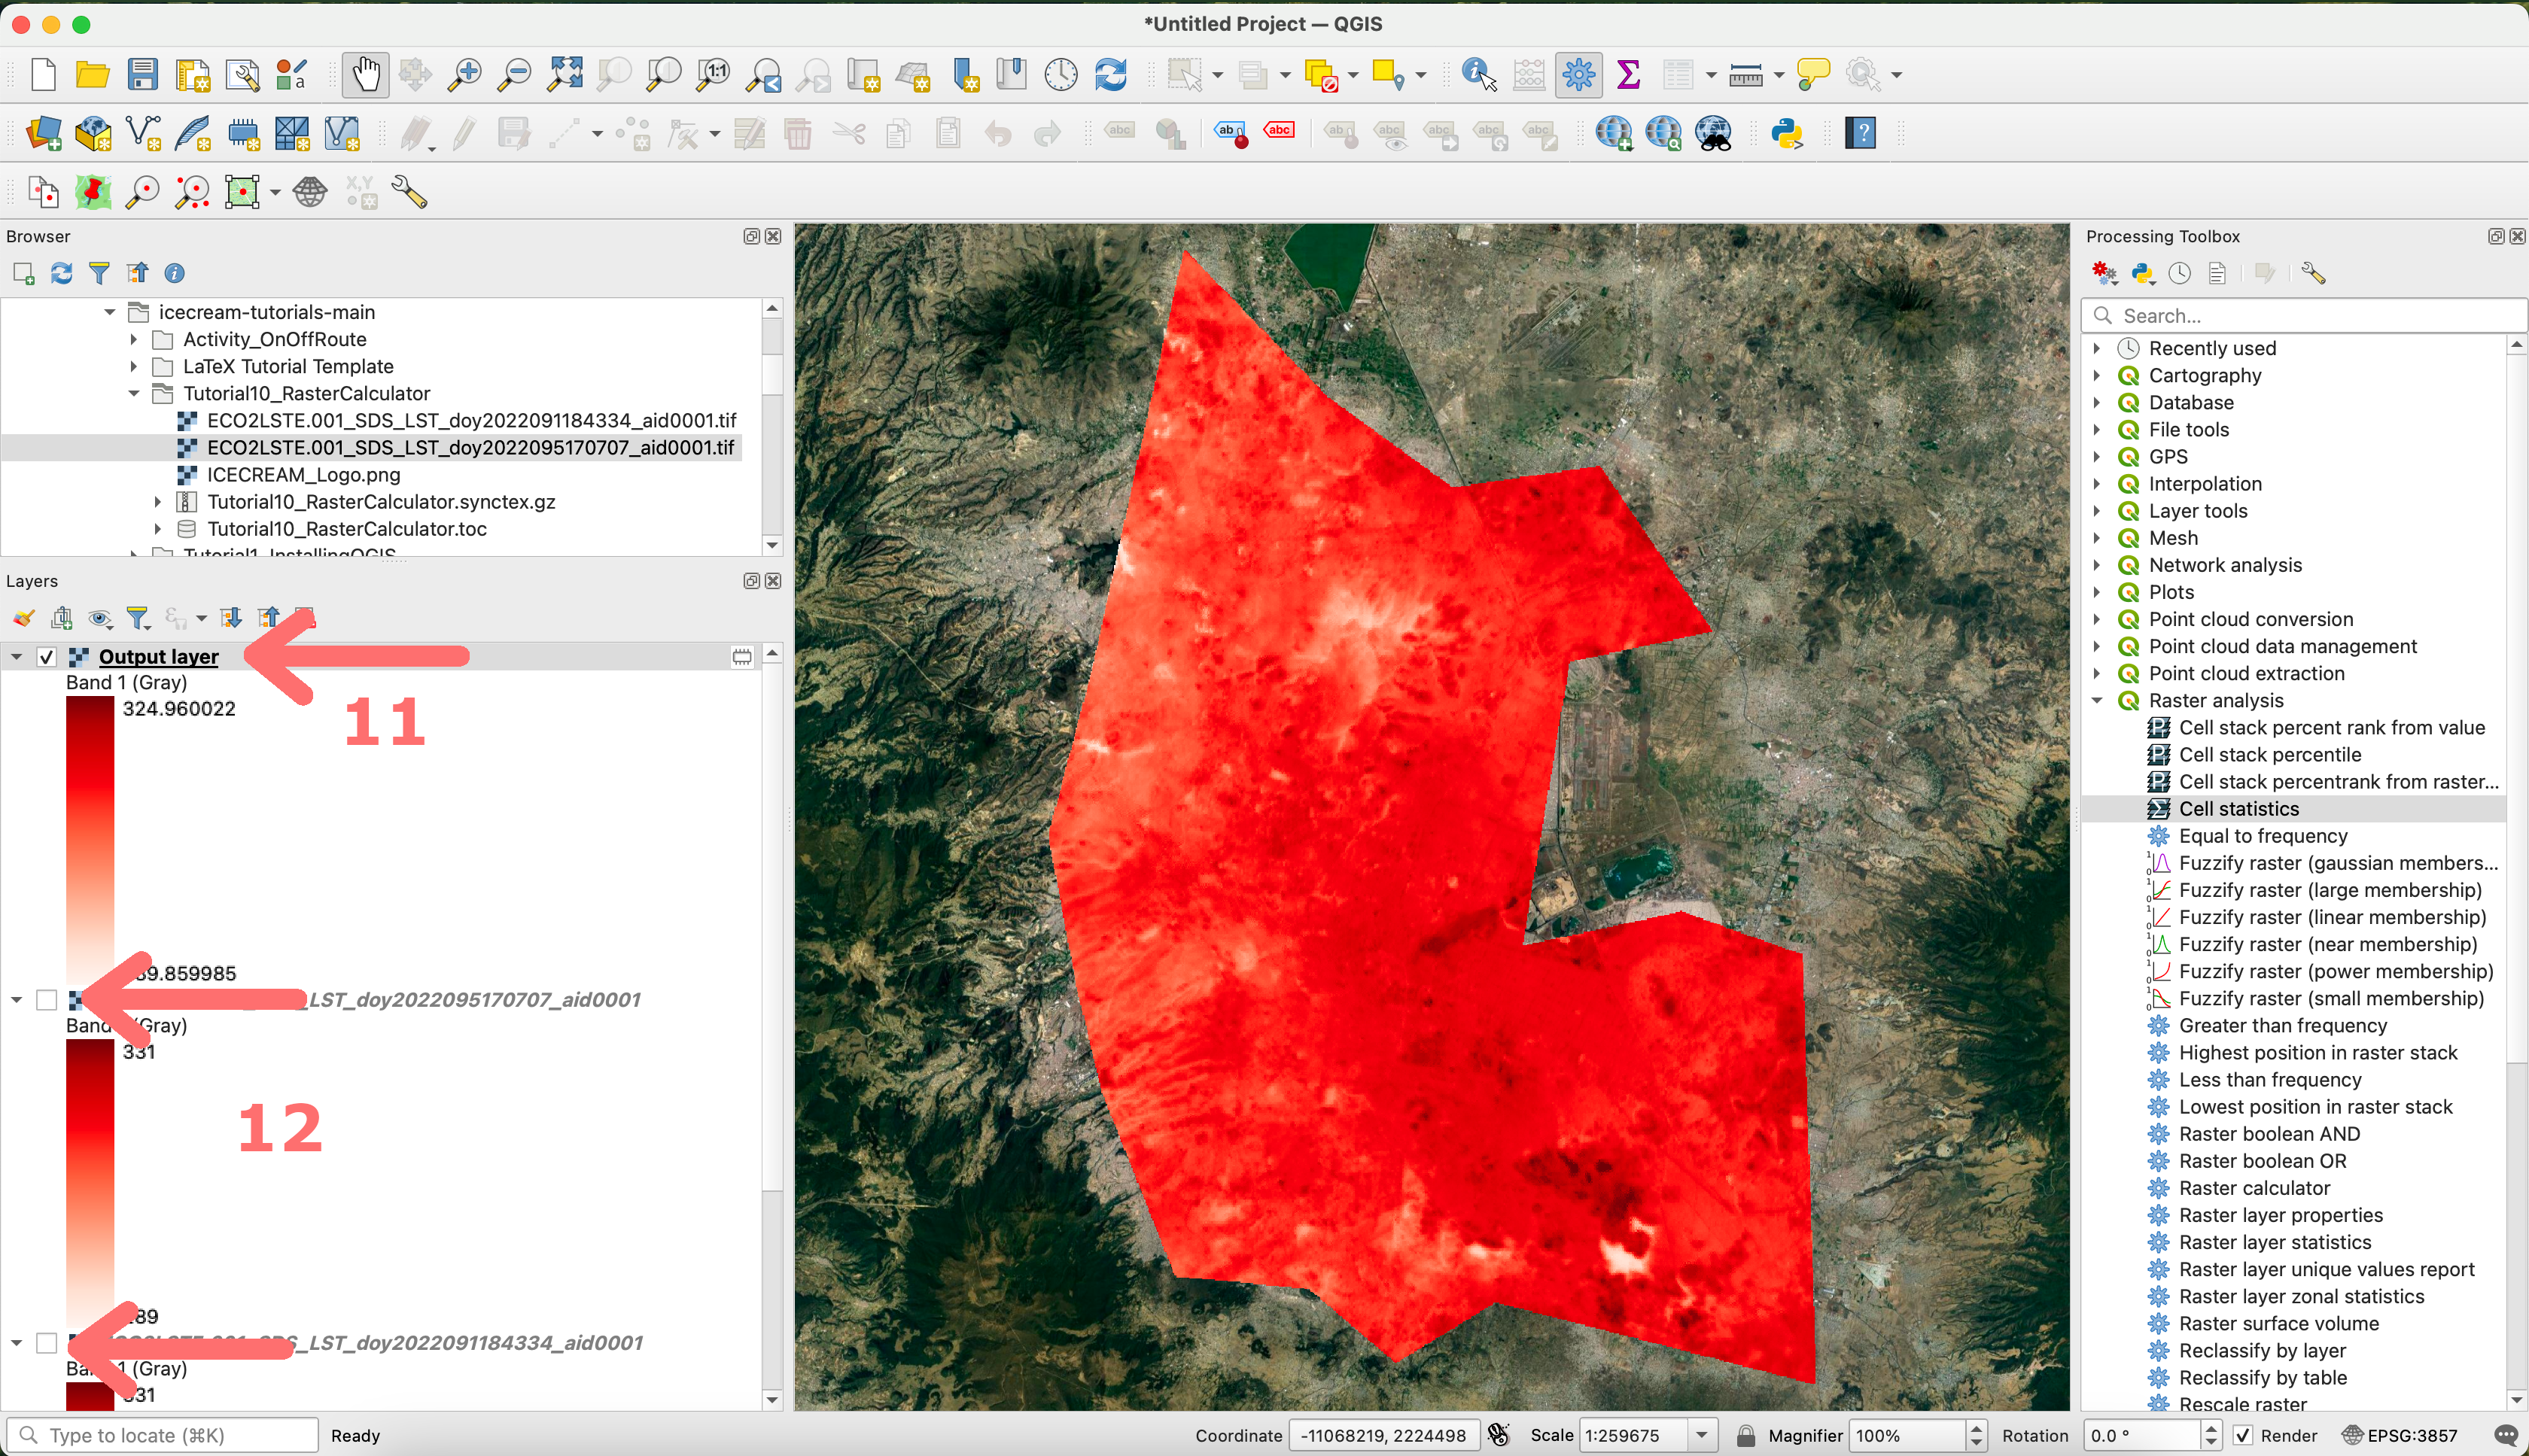
\includegraphics[width=\textwidth]{CellOutput.png}}

\vspace{.5em}

11. You now have a new layer that is the mean land surface temperature of the two GeoTIFFs for Mexico City.

12. To visualize this mean, deselect the other two layers. You can now change the color symbology and produce a map with this new layer. 

\kulbox{\textbf{NOTE:} This new layer can be exported as a GeoTIFF by right-clicking (ctrl-click on Mac) and clicking \textit{Save as...}. You can even use these output layers to create new layers with the same process. Maybe you want to look at the difference between the mean land surface temperatures of August 2022 and August 2023 for Death Valley. You can string together multiple mathematical operations to achieve this goal!}

\section{Using the Raster Calculator for Analyses}

13. Another compelling feature of raster math is the ability to make calculations. For example, there is quite a large swing in temperature between the days and nights. Let's use a more advanced feature of QGIS to calculate the \% difference in land surface temperature between an ECOSTRESS pass during the daylight hours and one deep into the night.

14. Download the following GeoTIFF files that show the land surface temperatures from two consecutive ECOSTRESS passes over Mexico City in February 2024. Save it somewhere you can remember and then add it as a layer in QGIS. Before starting, you may want to unclick the boxes of your other layers, leaving only your base map. Those other layers remain available later if you want to re-visualize them. 

\begin{itemize}
    \item \href{https://jeremydforsythe.github.io/icecream-tutorials/Tutorial11_RasterCalculator/ECO2LSTE.001_SDS_LST_doy2024049201450_aid0001.tif}{\small ECO2LSTE.001\_SDS\_LST\_doy2024049201450\_aid0001.tif}
    \item \href{https://jeremydforsythe.github.io/icecream-tutorials/Tutorial11_RasterCalculator/ECO2LSTE.001_SDS_LST_doy2024053084633_aid0001.tif}{\small ECO2LSTE.001\_SDS\_LST\_doy2024053084633\_aid0001.tif}
\end{itemize}

\underline{Recall the filenaming convention:}

    $<$\textbf{ProductShortName}$>$ ................ ECO2LSTE \\
    $<$\textbf{Version}$>$ ................ 001  \\
    $<$\textbf{LayerName}$>$ ................ SDS\textunderscore LST \\
    $<$Year$>$ ................ 2024  \\
    $<$\textbf{JulianDate} \& \textbf{Time}$>$ ................ doy2024049201450  \\
    $<$\textbf{AppEEARSFeatureID}$>$ ................ aid0001 \\
    $<$\textbf{FileFormat}$>$ ................ tif

\vspace{.5em}

This means that the first file is from 2024, day of year 049, time in HH:MM:SS 20:14:50. Using your \href{https://jeremydforsythe.github.io/icecream-tutorials/Tutorial4_AccessingRemoteSensingDataWithAppears/Julian_Calendar.png}{Julian Calendar} you know that day 49 is February 18, 2024. Your knowledge of military time reminds you that 20:14:50 is just before 8:15 pm UTC time. Also, you know from \href{https://jeremydforsythe.github.io/icecream-tutorials/Tutorial11_RasterCalculator/World_Time_Zones_Map.png}{this World Time Zone Map} that Mexico City is -6 hours from UTC, making the first file (ECO2LSTE.001\_SDS\_LST\_doy2024049201450\_aid0001.tif) about 2:15 pm in the afternoon local time. The same process reveals the second file \\(ECO2LSTE.001\_SDS\_LST\_doy2024053084633\_aid0001.tif) to be from 2:46am local time just a few days later on February 22, 2024. 

15. To calculate the \% difference in land surface temperature from night to day, we will use this formula:

\begin{equation}
    \left(\frac{(Day - Night)}{Night}\right) * 100
\end{equation}

in the \textit{Raster Calculator}. 

First, change the scales of the two GeoTIFF layers you imported in Step 14 to the same temperature range. This will help you understand the difference between daytime and nighttime temperatures. I used a minimum of 270 Kelvin and a maximum of 320 Kelvin in a ``Singleband Pseudocolor'' Render Type with the ``Reds'' color ramp. Refer to \href{https://jeremydforsythe.github.io/icecream-tutorials/Tutorial5_VisualizingDataWithQGIS/Tutorial5_VisualizingDataWithQGIS.pdf}{Tutorial \# 5 : Visualizing Data with QGIS} if you need a refresher on symbology.

16. From the menu bar, click on \textit{Raster}, then \textit{Raster Calculator}.

17. Check the box next to ``Create on-the-fly raster instead of writing to the disk''. This will create a layer in your layer window, but not save a brand new GeoTIFF to your computer's storage. For more complex operations or if you wanted to permanently save the results of the raster calculator, you would leave this unchecked and instead pick a location on your computer to store the new GeoTIFF. 

18. Name the resulting layer something useful, I picked ``PercentDifference''.

19. Use the \textit{Raster Bands}, \textit{Operators}, and \textit{Raster Calculator Expression} windows to enter the \% difference formula.

Begin with two open parentheses \textit{(} from the operator window. Then double-click the daytime raster. Follow with the \textit{-} operator, a double-click on the nighttime raster, the \textit{)/} operators, a double-click of the nighttime raster, the \textit{)*} operators, and then type the number 100.

\kulbox{\textbf{NOTE:} You could attempt to type out this formula in the expression box, but I find the raster calculator to be unforgiving to mistakes, so I recommend using the double-click method for the layers, and using the operator buttons.}

\vspace{.5em}

\centerline{\includegraphics[width=\textwidth]{RasterCalc.png}}

\vspace{.5em}

20. When you have finished, click the \textit{OK} button, and QGIS will compute the raster math and create a new on-the-fly layer for you. Look for the new layer in the \textit{Layers} window.

\kulbox{\textbf{NOTE:} You are probably noticing that the computed raster layer is looking pretty wonky. This is because of the irregular shape of our ECOSTRESS raster file. QGIS has drawn an arbitrary box around our jagged edged raster layer, with values for each cell. The values outside of our Mexico City boundary are not meaningful and will be filtered out in the next step.}

21. We need to do some cleaning of our percent difference layer so it communicates what we want it to. Double click on the ``Percent Difference'' layer in the \textit{Layers} panel (or control-click / right-click and select properties). 

22. Select \textit{Symbology}.

23. Change \textit{Render Type} to ``Singleband pseudocolor''. 

24. Change the color ramp to ``Reds'' by using the small down arrow to the right of the end of the Color Ramp input section, if it is not already the default. 

25. Change the \textit{Min} and \textit{Max} values to 0 and 17 to cover the range of values we have for the percent difference. 

\centerline{\includegraphics[width=\textwidth]{PercentDifferenceLayer.png}}

\vspace{.5em}

26. QGIS has automatically binned the values and assigned a corresponding color across the red gradients. However, the value of 0 only exists outside of our Mexico City boundary, so let's make it transparent. Double-click on the color square for the \textit{Value} of ``0''.

27. Move the \textit{Opacity} slider all the way to the left for 0\%. This will make all values of 0 transparent.

28. Click ``OK'' in both windows. Now you have a map showing which parts of Mexico City have the least and greatest temperature swing from night to day. 

\vspace{.5em}

\centerline{\includegraphics[width=\textwidth]{PercentDifferenceFinal.png}}

\begin{tcolorbox}[colback=yellow!5!white,colframe=MACred,title= \vspace{.2em} \Large Make a Map Assignments]
	\addcontentsline{toc}{section}{Make A Map Assignments}
	\large
	\begin{enumerate}
		\item Make a map for an area of interest that uses raster math to try and improve your ability to answer a question. You could use any ECOSTRESS product (land surface temperature, evapotranspiration, water-use efficiency, or evaporative stress index) to calculate a difference, a sum, or an average. The most important part of this exercise is to engage raster math as a way of better addressing your question. 
		\item Find a classmate and compare maps. Is your classmate doing anything differently that can help improve your map? If so, revise accordingly! 
            \item Submit your map with raster math applied, along with a short description. In particular, your description might address any interesting observations and address any limitations of your analysis.
	\end{enumerate}
\end{tcolorbox}

\begin{tcolorbox}[colback=yellow!5!white,title=\textbf{Datafiles}]
	\addcontentsline{toc}{section}{Datafiles}
	\large
	Here are links to the ECOSTRESS LST GeoTIFF files for Mexico City used in this tutorial:

    \begin{enumerate}
        \item \href{https://jeremydforsythe.github.io/icecream-tutorials/Tutorial11_RasterCalculator/ECO2LSTE.001_SDS_LST_doy2022091184334_aid0001.tif}{\small ECO2LSTE.001\_SDS\_LST\_doy2022091184334\_aid0001.tif}
        \item \href{https://jeremydforsythe.github.io/icecream-tutorials/Tutorial11_RasterCalculator/ECO2LSTE.001_SDS_LST_doy2022091184334_aid0001.tif}{\small ECO2LSTE.001\_SDS\_LST\_doy2022091184334\_aid0001.tif}
        \item \href{https://jeremydforsythe.github.io/icecream-tutorials/Tutorial11_RasterCalculator/ECO2LSTE.001_SDS_LST_doy2024049201450_aid0001.tif}{\small ECO2LSTE.001\_SDS\_LST\_doy2024049201450\_aid0001.tif}
        \item \href{https://jeremydforsythe.github.io/icecream-tutorials/Tutorial11_RasterCalculator/ECO2LSTE.001_SDS_LST_doy2024053084633_aid0001.tif}{\small ECO2LSTE.001\_SDS\_LST\_doy2024053084633\_aid0001.tif}
        \item And my Mexico City shapefile: \href{https://jeremydforsythe.github.io/icecream-tutorials/Tutorial10_ESI/MexicoCityPolygon/MexicoCity.geojson}{\small MexicoCity.geojson}
    \end{enumerate}
\end{tcolorbox}

%%%%%%%%%%%%%%%%%%%%%%%%%%%%%%%%%%%%%%%%%%%%%%%%%%%%%%%%%%%%%%%%%%%%%%%%%%%%%%%%%%% End of Document
\vfill

\hrule

\vspace{1em}

\small \textbf{Recommended Citation:} Forsythe, J.D., G.R. Goldsmith, and J.B. Fisher. 2023. Observing Earth from Above Tutorials. Chapman University. \url{https://jeremydforsythe.github.io/icecream-tutorials/}

\vspace{1em}

This work is supported by funding from NASA ECOSTRESS Mission Grant \#80NSSC23K0309 (I.C.E. C.R.E.A.M.: Integrating Communication of ECOSTRESS Into Community Research, Education, Applications, and Media) and is openly licensed via \href{https://creativecommons.org/licenses/by-nc/4.0/}{CC BY-NC}.

\end{document}
